%%
%% Copyright 2022 OXFORD UNIVERSITY PRESS
%%
%% This file is part of the 'oup-authoring-template Bundle'.
%% ---------------------------------------------
%%
%% It may be distributed under the conditions of the LaTeX Project Public
%% License, either version 1.2 of this license or (at your option) any
%% later version.  The latest version of this license is in
%%    http://www.latex-project.org/lppl.txt
%% and version 1.2 or later is part of all distributions of LaTeX
%% version 1999/12/01 or later.
%%
%% The list of all files belonging to the 'oup-authoring-template Bundle' is
%% given in the file `manifest.txt'.
%%
%% Template article for OXFORD UNIVERSITY PRESS's document class `oup-authoring-template'
%% with bibliographic references
%%

%%%CONTEMPORARY%%%
%\documentclass[unnumsec,webpdf,contemporary,large]{oup-authoring-template}%
%\documentclass[unnumsec,webpdf,contemporary,large,namedate]{oup-authoring-template}% uncomment this line for author year citations and comment the above
%\documentclass[unnumsec,webpdf,contemporary,medium]{oup-authoring-template}
%\documentclass[unnumsec,webpdf,contemporary,small]{oup-authoring-template}

%%%MODERN%%%
\documentclass[unnumsec,webpdf,modern,large]{oup-authoring-template}
%\documentclass[unnumsec,webpdf,modern,large,namedate]{oup-authoring-template}% uncomment this line for author year citations and comment the above
%\documentclass[unnumsec,webpdf,modern,medium]{oup-authoring-template}
%\documentclass[unnumsec,webpdf,modern,small]{oup-authoring-template}

%%%TRADITIONAL%%%
%\documentclass[unnumsec,webpdf,traditional,large]{oup-authoring-template}
%\documentclass[unnumsec,webpdf,traditional,large,namedate]{oup-authoring-template}% uncomment this line for author year citations and comment the above
%\documentclass[unnumsec,namedate,webpdf,traditional,medium]{oup-authoring-template}
%\documentclass[namedate,webpdf,traditional,small]{oup-authoring-template}

%\onecolumn % for one column layouts

%\usepackage{showframe}
\usepackage{graphicx}	% Including figure files
\usepackage{amsmath}	% Advanced maths commands
\usepackage{amssymb}	% Extra maths symbols
\usepackage{mathtools}
\usepackage{hyperref}
\usepackage{natbib}
\usepackage{caption}
%\usepackage{subcaption}
\captionsetup{compatibility=false}
\usepackage{gensymb}
%\usepackage{enumitem}
\usepackage{newtxtext,newtxmath}
\usepackage{booktabs}

% line numbers
%\usepackage[mathlines, switch]{lineno}
%\usepackage[right]{lineno}

\begin{document}
	
	\journaltitle{Journal Title Here}
	\DOI{DOI HERE}
	\copyrightyear{2024}
	\pubyear{2024}
	\access{Advance Access Publication Date: Day Month Year}
	\appnotes{Paper}
	
	\firstpage{1}
	
	%\subtitle{Subject Section}
	
	\title[Finding multiplets]{More cells, more doublets in sample-barcoded single-cell data}
	
	\author[1, 2]{George Howitt}
	\author[1, 2]{Gunjan Dixit}
	\author[1,2]{Rotem Aharon}
	\author[1]{Victoria Streeton-Cook}
	\author[3]{Ling Ling}
	\author[3,4]{Peter F. Hickey}
	\author[3,4]{Daniela Amann-Zalcenstein}
	\author[5]{Liam Gubbels}
	\author[5,6,7]{Shivanthan Shanthikumar}
	\author[5,6,7]{Sarath Ranganathan}
	\author[5,6]{Melanie Neeland}
	\author[1, 2]{Jovana Maksimovic}
	\author[1, 2, 8,$\ast$]{Alicia Oshlack}
	
	\authormark{Howitt et al.}
	
	\address[1]{Computational Biology Program, Peter MacCallum Cancer Centre, Parkville, VIC, Australia}
	\address[2]{Sir Peter MacCallum Department of Oncology, University of Melbourne, Parkville, VIC, Australia}
	\address[3]{The Walter and Eliza Hall Institute of Medical Research, Parkville, VIC 3052, Australia}
	\address[4]{Department of Medical Biology, University of Melbourne, Parkville, VIC, Australia}
	\address[5]{Respiratory Diseases, Murdoch Children’s Research Institute, Parkville, VIC, Australia}
	\address[6]{Respiratory and Sleep Medicine, Royal Children’s Hospital, Parkville, VIC, Australia}
	\address[7]{Department of Paediatrics, University of Melbourne, Parkville, VIC, Australia}
	\address[8]{School of Mathematics and Statistics, University of Melbourne, Parkville, VIC, Australia}
		
	\corresp[$\ast$]{alicia.oshlack@petermac.org}
		
	\received{Date}{0}{Year}
	\revised{Date}{0}{Year}
	\accepted{Date}{0}{Year}
	
	%\editor{Associate Editor: Name}
	
	%\abstract{
		%\textbf{Motivation:} .\\
		%\textbf{Results:} .\\
		%\textbf{Availability:} .\\
		%\textbf{Contact:} \href{name@email.com}{name@email.com}\\
		%\textbf{Supplementary information:} Supplementary data are available at \textit{Journal Name}
		%online.}
	
	\abstract{
		Sample barcoding allows deconvolution of multiplets in multiplexed droplet-based single-cell RNA-sequencing experiments. 
		However, this is only possible when each cell comes from a different sample. As the number of cells in a droplet increases, the probability of two or more cells coming from the same sample increases rapidly. 
		We show that the number of these unresolvable multiplets is greater than previously estimated for the 10X Flex scRNA-seq protocol, and provide a formula for estimating the fraction of multiplets in a data set given a measured average droplet occupancy and number of unique samples in a pool. 
		We also show that existing doublet detection tools should be applied to Flex data to identify these multiplets, and demonstrate that filtering out barcodes identified by these tools improves downstream analysis.		 	
		}
	%\keywords{}
	
		\maketitle

		\section{Introduction}
	\label{sec:introduction}
	
	As single-cell RNA-sequencing (scRNA-seq) experiments grow in scale, performing separate captures for individual samples becomes prohibitively expensive. 
	Pooling multiple samples in a single experiment both reduces cost and minimises batch effects, but introduces a new problem – how to associate individual cells with their sample of origin. 
	A common method involves tagging the samples with either antibody or lipid-linked unique oligo barcodes prior to pooling. 
	These ``hashtag'' oligos attach to either proteins
	\citep{Stoeckius2018} 
	or lipids \citep{McGinnis2019}
	on the cell surface and can be sequenced along with the gene expression, and various methods have been developed to identify the sample of origin from the expression counts of the hashtags 
	\citep{Howitt2023}.
	However, hashtag-based multiplexing has several drawbacks. 
	Firstly, tagging introduces an additional step into the sample preparation workflow, and may be more challenging for certain tissue types. 
	Poor staining can cause many cells to be unidentifiable, even when the underlying RNA expression data is high quality 
	\citep{Brown2024}. 
re, especially for poor quality hashtagging 
	\citep{Howitt2023}.
	
	In droplet-based scRNA-seq protocols, cells are encapsulated within droplets which contain oligo barcoded beads that hybridise to each RNA molecule in the cell. 
	This allows for the allocation of reads to droplets, and, assuming each droplet contains either zero or one cell, each read can be associated with a single cell. 
	If droplets contain two or more cells (called doublets, or more generally multiplets), the RNA expression from all the cells is pooled together in the expression counts matrix, creating artifacts which may be erroneously identified as novel or transitional cell types. 
	While multiplets can be identified based on their  RNA expression profiles or using hashtags, they must be discarded from any downstream analysis
	\citep{Neavin2024}.
	Therefore, excessive numbers of multiplets are a major concern in droplet-based scRNA-seq experiments, particularly as the main approach for  avoiding them is to reduce the capture throughput, thereby producing many more empty than cell-containing droplets, which in turn increases costs.
	
	The Flex protocol from 10X Genomics addresses both of the above issues by using barcoded gene-specific probes that hybridise to individual RNA molecules in the cell. 
	These barcodes can include an oligo that identifies a specific sample, with available kits containing 4 and 16 unique sample barcodes. 
	The uniquely barcoded gene probes are added to each sample prior to pooling. 
	Probe hybridisation is then followed by encapsulation within droplets containing GEMs (Gel beads-in-emulsion) similar to other 10X droplet-based protocols. 
	After sequencing, each read then includes a barcode from both the sample of origin as well as the droplet, allowing immediate demultiplexing of pooled samples and resolution of multiplets from distinct samples within the same droplet. 
	This removes the need for separate hashtag-staining and demultiplexing steps in the scRNA-seq workflow, and the resolution of multiplets allows for higher throughput in the library preparation stage. 
	Consequently, according to the manufacturer, up to 128,000 cells from up to 16 samples can be run on a single lane of a Chromium X instrument 
	\citep{10X_flex_protocol}. 
	
	However, while cells from different samples in the same droplet can be resolved with Flex, cells from the same sample remain unresolvable, and the number of these increases steeply with the occupancy of droplets. 
	This is analogous to the ``birthday paradox” in classical probability, where the probability of two people in a room sharing the same birthday increases faster than expected by intuition, as the number of people in the room increases
	\citep{Mulqueen2021}.
	Here we demonstrate that the number of multiplets found in real Flex data is significantly higher than initially expected, and describe a mathematical model for estimating the number of multiplets that is closer to the observed value. 

	\section{Results}
	\label{sec:results}
	
	\subsection{Flex data sets}
	\label{subsec: data}
	
	We perform our analysis using two data sets acquired from ten 16-plex Flex runs. 
	The first data set, the earlyAIR data set, comes from an ongoing study to create a single-cell atlas of the paediatric airway, and comprises nine 16- plex batches from five tissue types, comprising both solid and liquid tissues from healthy donors. 
	Some donors provided multiple tissues, and the batches contain between 25,486 and 139,926 cells after pre-processing (see Methods). 
	The second data set, the PBMC data set, comprises 16 replicates of peripheral blood mononuclear cells taken from a healthy donor and is publicly available from 10X Genomics (see Data availability).  
	The PBMC data set contains 135,785 cells after pre-processing.
	
	\subsection{Verification of doublet finders with known multiplets}

	Tests of doublet-finding methods have to date relied upon a ground truth determined from alternative experiments, such as genotype information 
	\citep{Neavin2024},
	hashtag-based demultiplexing 
	\citep{Curion2024}, 
	DNA barcoding \citep{Zhang2024}, 
	or synthetic data 
	\citep{Xi2021}.	
	Flex allows for a novel means of testing doublet finding directly using the RNA sequencing output. 
	In a Flex experiment, due to superloading, many droplets contain multiple cells and cell calling is performed separately for each sample barcode. 
	This means the initial step in a standard Flex analysis is to separate reads based on their combined droplet and sample barcode and then call cell-containing or empty ``droplets" based on the data separated by samples. 
	A droplet/sample combination may look empty even when there is a ``cell" from a different sample in the same droplet. 
	The resulting counts matrix has cells labeled by both the droplet barcode and sample barcode. 
	Aggregating the counts for each ``droplet” across the sample barcodes creates a droplet-level counts matrix analogous to 3’ scRNA-seq experiments. 
	Since the number of cells (from unique samples) called by CellRanger in each droplet is known, the droplet-level counts matrix provides a ground truth data set for testing doublet finders: droplets with only one cell are singlets and droplets with two or more cells are doublets. 
	Note, this section is not intended as a comprehensive benchmark of doublet-finding methods, which may be found in 
	\citep{Neavin2024}. 
	Instead, we apply two of the best-performing packages with low computational overhead recommended in 
	\citep{Neavin2024}: 
	scds 
	\citep{Bais2020} 
	and scDblFinder 
	\citep{Germain2021} 
	and evaluate which performs best on our Flex data sets. 
	scds has two methods for doublet detection, one based on marker co-expression and another based on binary classification, as well as a hybrid classifier that combines both methods. 
	We use all approaches and some details of how each method works and the parameters chosen can be found in the Methods section. 
		
	Figure \ref{fig:doublet_finder_comparison} shows the performance of scDblFinder and the two scds methods as well as the hybrid classifier on the droplet-aggregated 10X PBMC data set.	 
	%
	\begin{figure}
		\begin{center}
			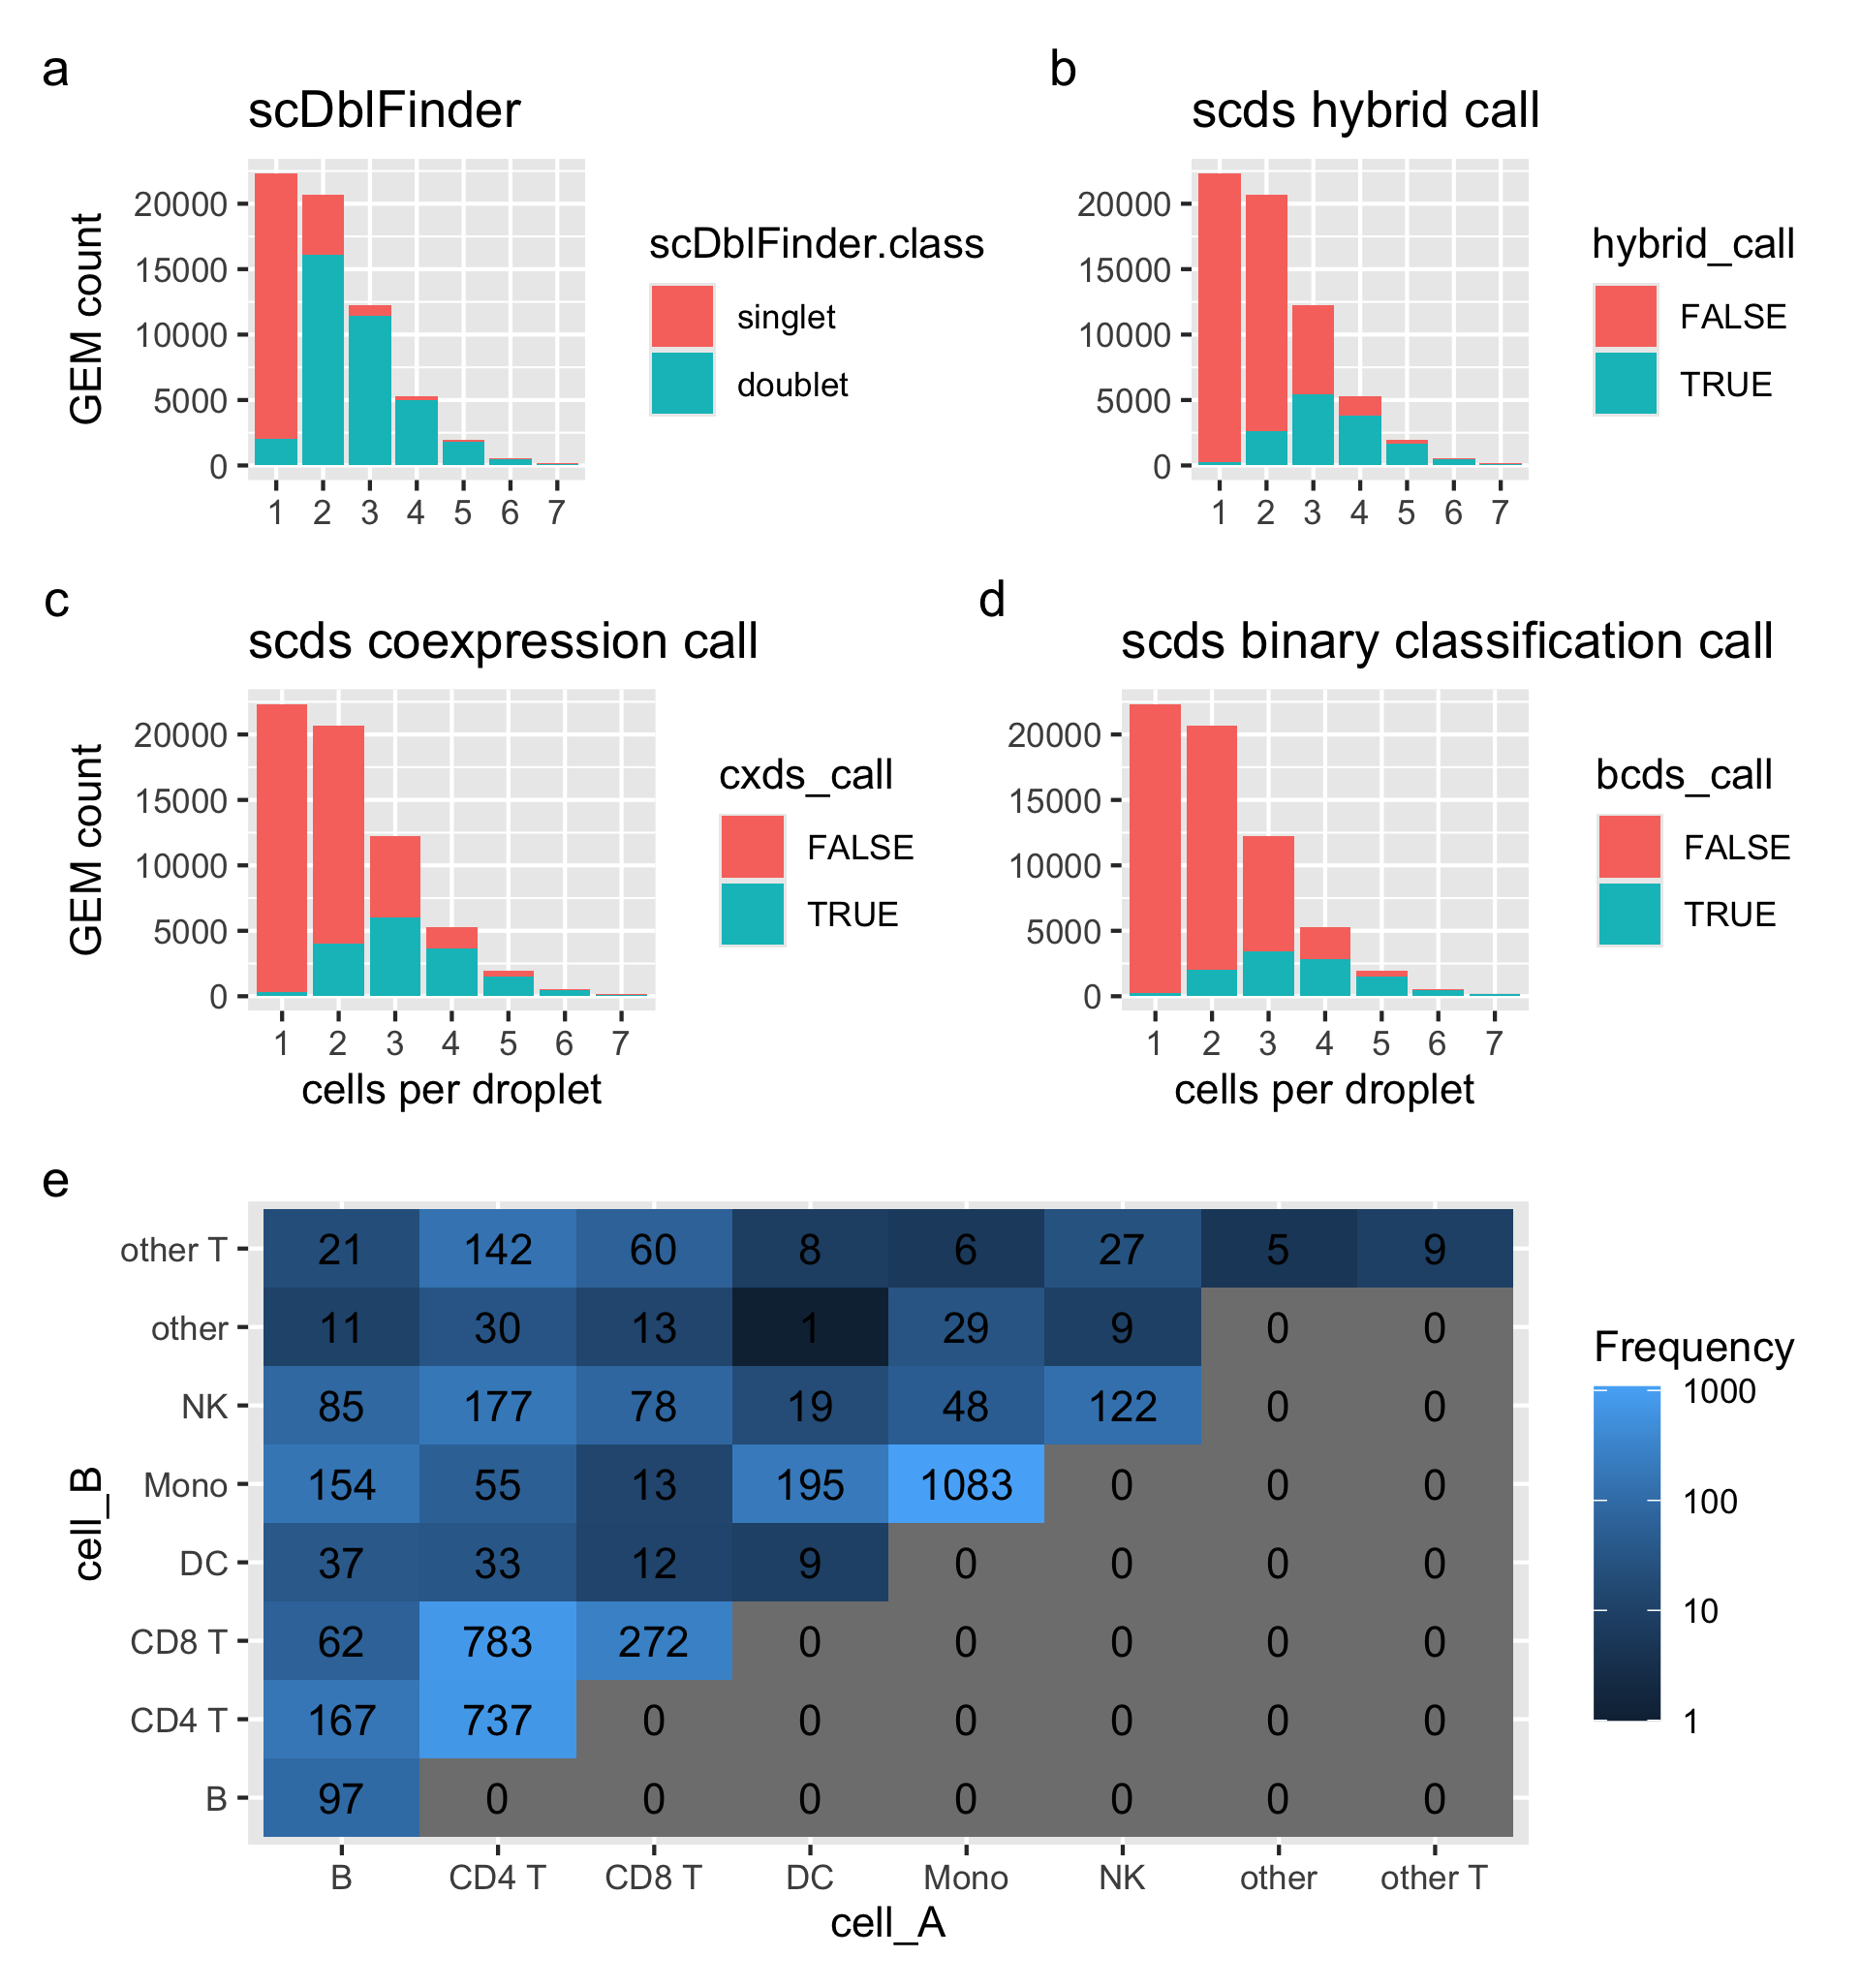
\includegraphics[scale=0.08 ]{figures/doublet_finder_comparison_extra.png} 
			\caption{ a)-d) Performance of doublet-finders on droplets with occupancy determined by CellRanger calls. 
			Each bar represents the identified number of cells in a droplet based on the sample deconvolution. 
			The blue portion represents the number of detected doublets from the doublet detection tool.
			Ideally, a tool will only detect singlets where there is one cell per droplet and doublets when there is more than one cell.  
			e) Cell type composition of droplets containing two cells called by CellRanger which are called singlets by scDblFinder. The majority (>50\%) of cells misclassified as singlets are homotypic doublets.
			}
			\label{fig:doublet_finder_comparison}
		\end{center}
	\end{figure}
	%
	For this data, scDblFinder (Figure \ref{fig:doublet_finder_comparison}a) clearly outperforms the scds methods (Figure \ref{fig:doublet_finder_comparison} b-d), with 90\% of the multiply-occupied droplets called as doublets compared to only 25\%-40\%. 
	22\% of droplets containing two cells are called singlets by scDblFinder. 
	Doublet-finding methods are known to perform poorly on droplets containing multiple cells of the same type (homotypic doublets), as these are unlikely to show discrepant transcription profiles
	\citep{Xiong2022, Neavin2024}.
	We use the reference mapping package Azimuth and its included PBMC reference data set to annotate the PBMC data set
	\citep{Hao2021},
	and examine the composition of the unidentified doublets. 	
	Figure \ref{fig:doublet_finder_comparison}e) shows that the majority (50.5\%) are homotypic doublets, or have more closely related transcriptional profiles such as CD8+ T cells with CD4+ T cells (17\%).	
	scDblFinder calls 9.2\% of the CellRanger singlets as doublets, compared to < 2\% for scds. 
	In the following sections, we examine doublets in more depth and show that the rate of unresolved doublets predicted by our mathematical model is quite close to the value from scDblFinder.
	
	\subsection{Measuring multiplet rates in Flex data}
	
	Having identified scDblFinder 
	\citep{Germain2021}
	as our preferred doublet-finding method for this study, we apply it to all of our data sets. 
	Figure \ref{fig:doublet rate 16-plex} shows the fraction of doublets called by scDblFinder on each Flex run as a function of the number of cells.
	%
	\begin{figure}
		\begin{center}
			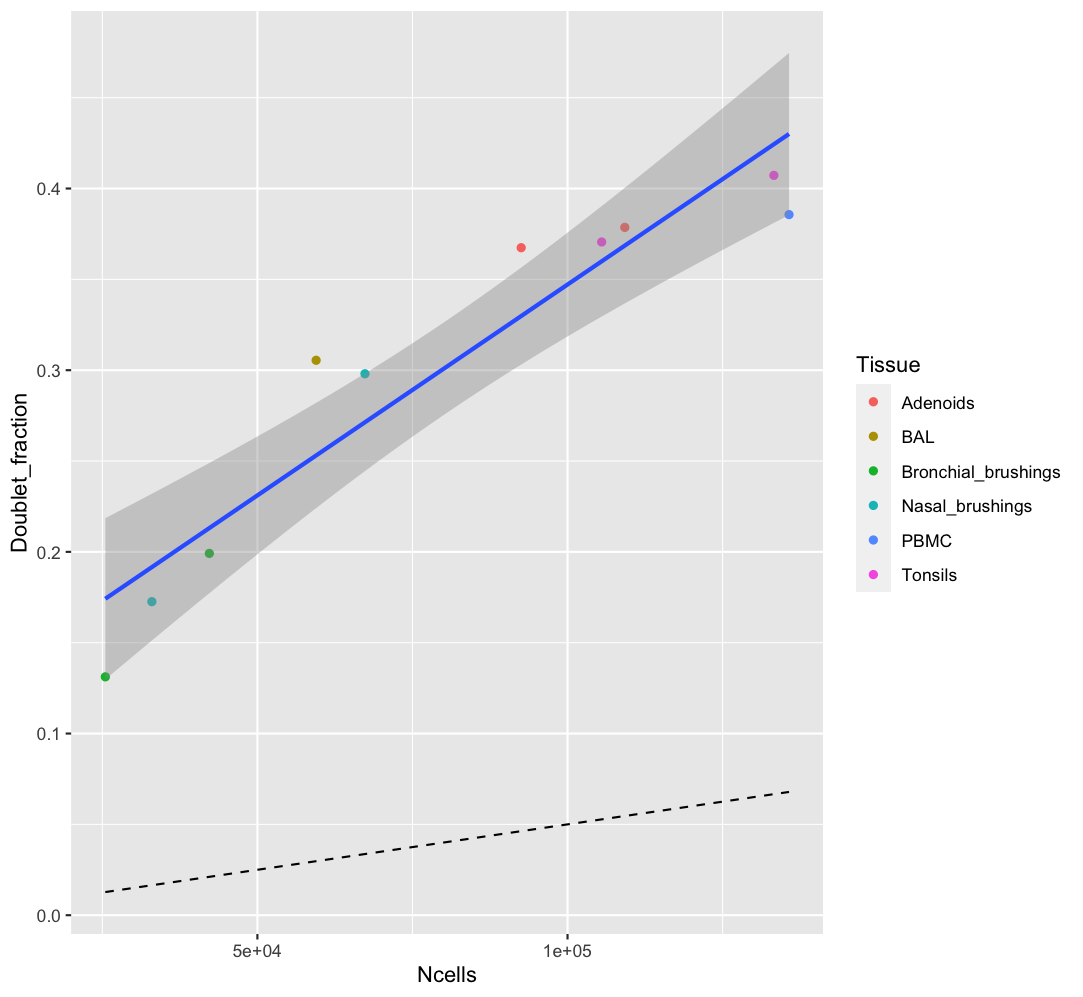
\includegraphics[scale=0.13]{figures/doublet_rate_16plex.png}	\\
			\caption{Doublet fraction (from scDblFinder) vs number of cells called for 10 16-plex Flex data sets. 
				The blue line indicates a linear fit to the data. 
				The black dashed line is the estimated rate from the Flex user guide. 
			}		
			\label{fig:doublet rate 16-plex}
		\end{center}
	\end{figure}
	%
	Also shown in Figure  \ref{fig:doublet rate 16-plex} is the predicted doublet fraction from the documentation for the Flex protocol 
	\citep{10X_flex_protocol}
	of 0.8\% per 1000 cells per sample, or 0.05\% per 1000 cells for 16-plex runs. 
	A clear linear trend is observed in the results from scDblFinder, with a best fit multiplet rate of 0.23\% per 1000 cells, or $\approx 4.6$ times more than the estimate from the documentation.
		
	\subsection{Estimating the resolvable cell fraction}
	\label{subsec:multiplet theory}
	
	Why is the multiplet rate predicted by doublet finders so much greater than the rate estimated by the manufacturer? 
	Recall that the quoted rate of unresolvable multiplets in Flex comes from dividing the rate for the 3' protocol by the number of samples. 
	This makes sense if each Flex sample is processed separately at the same concentration as an equivalent 3' sample, but the recommended practice is to pool all samples together after probe hybridisation, so that the concentration of cells is up to 16 times greater than a 3' experiment sequencing the same number of cells per sample. 
	3' experiments are designed to avoid multiplets, so that very few droplets contain more than one cell. 
	In Flex experiments the ability to resolve cells from different samples within the same droplet means that total cell concentrations can be much larger, and droplets containing multiple cells are common (cf. Figure \ref{fig:doublet_finder_comparison}). 
	In this section, we perform some calculations showing that increasing the occupancy of droplets leads to a higher number of unresolved cells than previously appreciated.
	
	Consider an ensemble of droplets containing $k$ cells, drawn from a pool containing $n$ samples with equal proportions of cells from all samples. 
	The number of possible configurations of cells within the droplets is the number of combinations of length $k$ drawn from $n$ with repetition allowed, i.e. 
	%
	\begin{equation}
		M_k(n) = \frac{(n + k - 1)!}{(n - 1)! k!} \quad ,
		\label{eq:multiplet_configurations}
	\end{equation}
	%
	where $!$ denotes the factorial function. 
	Assuming each of these combinations is equally probable, we aim to determine what fraction $F(n, k)$ of cells in droplets containing $k$ cells are ``resolvable'', which we define as being the only cell from their sample of origin.
	In general, 
	%
	\begin{equation}
		F(n, k) = \frac{\sum_{\mathrm c} f_{\mathrm c}}{M_k}
		\label{eq:resolvable_fraction_given_k}
	\end{equation}
	%
	where the subscript $\mathrm{c}$ denotes a single configuration of cells within a droplet, and $f_{\mathrm c}$ is the resolvable fraction of that configuration. 
	Compupting $F(n, k)$ therefore requires determining $f_c$ for each combination. 
	
	We define the observed occupancy of a droplet as $l$, $l \leq k$, as the number of unique samples in a droplet.
	Droplets with $k = 1$ are all resolvable.   
	For droplets with $k \geq 2$, if all cells in the droplet are from the same sample, i.e. $l=1$, no cells are resolvable, while if each cell comes from a unique sample, i.e. $l = k$, all cells are resolvable. 
	In general, we can use the concept of integer partition to determine the resolvable fraction of a given combination of cells.
	A partition is a way of writing an integer $k$ as a sum of integer ``parts'', e.g. the partitions of 5 are (5), (4 + 1), (3 + 2), (3 + 1 + 1), (2 + 2 + 1), (2 + 1 + 1 + 1), (1 + 1 + 1 + 1 + 1)
	\citep{Andrews1998}.
	In this framework, each part of the partition is a unique sample, the number of parts is the observed occupancy $l$, and the number of 1s in the partition is the number of resolvable cells, e.g., the partition (2 + 2 + 1) represents a droplet with $k$ = 5 consisting of 2 cells from sample A, 2 cells from sample B and 1 cell from sample C.
	We can define the fraction of resolvable cells in a droplet $f$ in two ways: first, the number of resolvable cells from unique samples in the droplet divided by the total number of cells in the droplet, i.e. the number of 1s in the partition divided by $k$; second, the number of resolvable cells divided by the number of unique samples in the droplet, i.e. the number of 1s in the partition divided by $l$. 
	Since we are interested in comparing to experimental data, we use the second definition.
	For the partitions of 5 written above, this gives $f = 0, 0.5. 0, 2/3, 1/3, 0.75, 1$.
	Since any configuration of cells within a droplet can be represented as a partition, and the resolvable fraction of each partition is easily calculable
	\citep{Andrews1998},
	 all that we need to solve \eqref{eq:resolvable_fraction_given_k} is the proportion each partition contributes to the total number of combinations $M_k$.
	 
	To begin, let's again consider the partition (2 + 2 + 1) representing 2 cells from sample A, 2 cells from sample B and 1 cell from sample C.
	There are $n$ possible choices for sample A. 
	If sample B is the same as sample A, then the droplet instead corresponds to the partition (4 + 1), so there are only $n-1$ choices for sample B, $n-2$ choices for sample C, and $n(n-1)(n-2)$ possible configurations for this partition. 
	
	In general, we denote each partition of $k$ $P_i(k)$.
	Define $m_j(P_i)$ the number of occurences of $j \in \lbrace 1, ..., k \rbrace$ in $P_i$.
	To determine the number of combinations corresponding to $P_i$, $C_i(n, k)$, consider the first non-zero $m_j$. 
	There are 
	$\binom{n}{m_j}$
	possible combinations of samples for these cells, where
	%
	\begin{equation}
		\binom {n}{m_j} = \frac{n!}{(n-m_j)! m_j!} \quad 
		\label{eq:combinations}
	\end{equation}
	%
	is the binomial coefficient. 
	For the next non-zero coefficient, $m_h$, there are only $n - m_j$ unique samples left to choose from, so the number of possible combinations is 
	$\binom{n-m_j}{m_h}$. 
	In general, we expect
	%
	\begin{equation}
		C_i(n, k) = \prod_{j=1}^{k} \binom{n - d_j}{m_j} \quad .
		\label{eq: partition combinations}
	\end{equation}
	%
	where 
	%
	\begin{equation}
		d_j = \sum_{h =1}^{j-1} m_h \quad ,
		\label{eq:chosen_sum}
	\end{equation}
	%
	with $d_0 = d_1 = 0$, is a variable that counts how many unique samples have already been chosen. 	
	As a check on \eqref{eq: partition combinations}, we find that 
	%
	\begin{equation}
		\sum_{i} C_i(n, k) = M_k(n)  
		\label{eq:continuity equation} 
	\end{equation}
	%
	as required. 
	Equation \eqref{eq:resolvable_fraction_given_k} then becomes 
	%
	\begin{equation}
		F(n, k) = \frac{ \sum_{i} f(P_i) C_i}{M_k} \, ,
		\label{eq:resolvable fraction}
	\end{equation}
	%
	where the observed occupancy, $l(P_i)$ is the length of the partition and the resolvable fraction of $P_i$, $f(P_i) = m_1(P_i) / l$.
	We show $F$ versus $k$ for $n = 4$ and $n = 16$ in Figure \ref{fig:resolvable_fraction}.	
	%
	\begin{figure}
		\begin{center}
			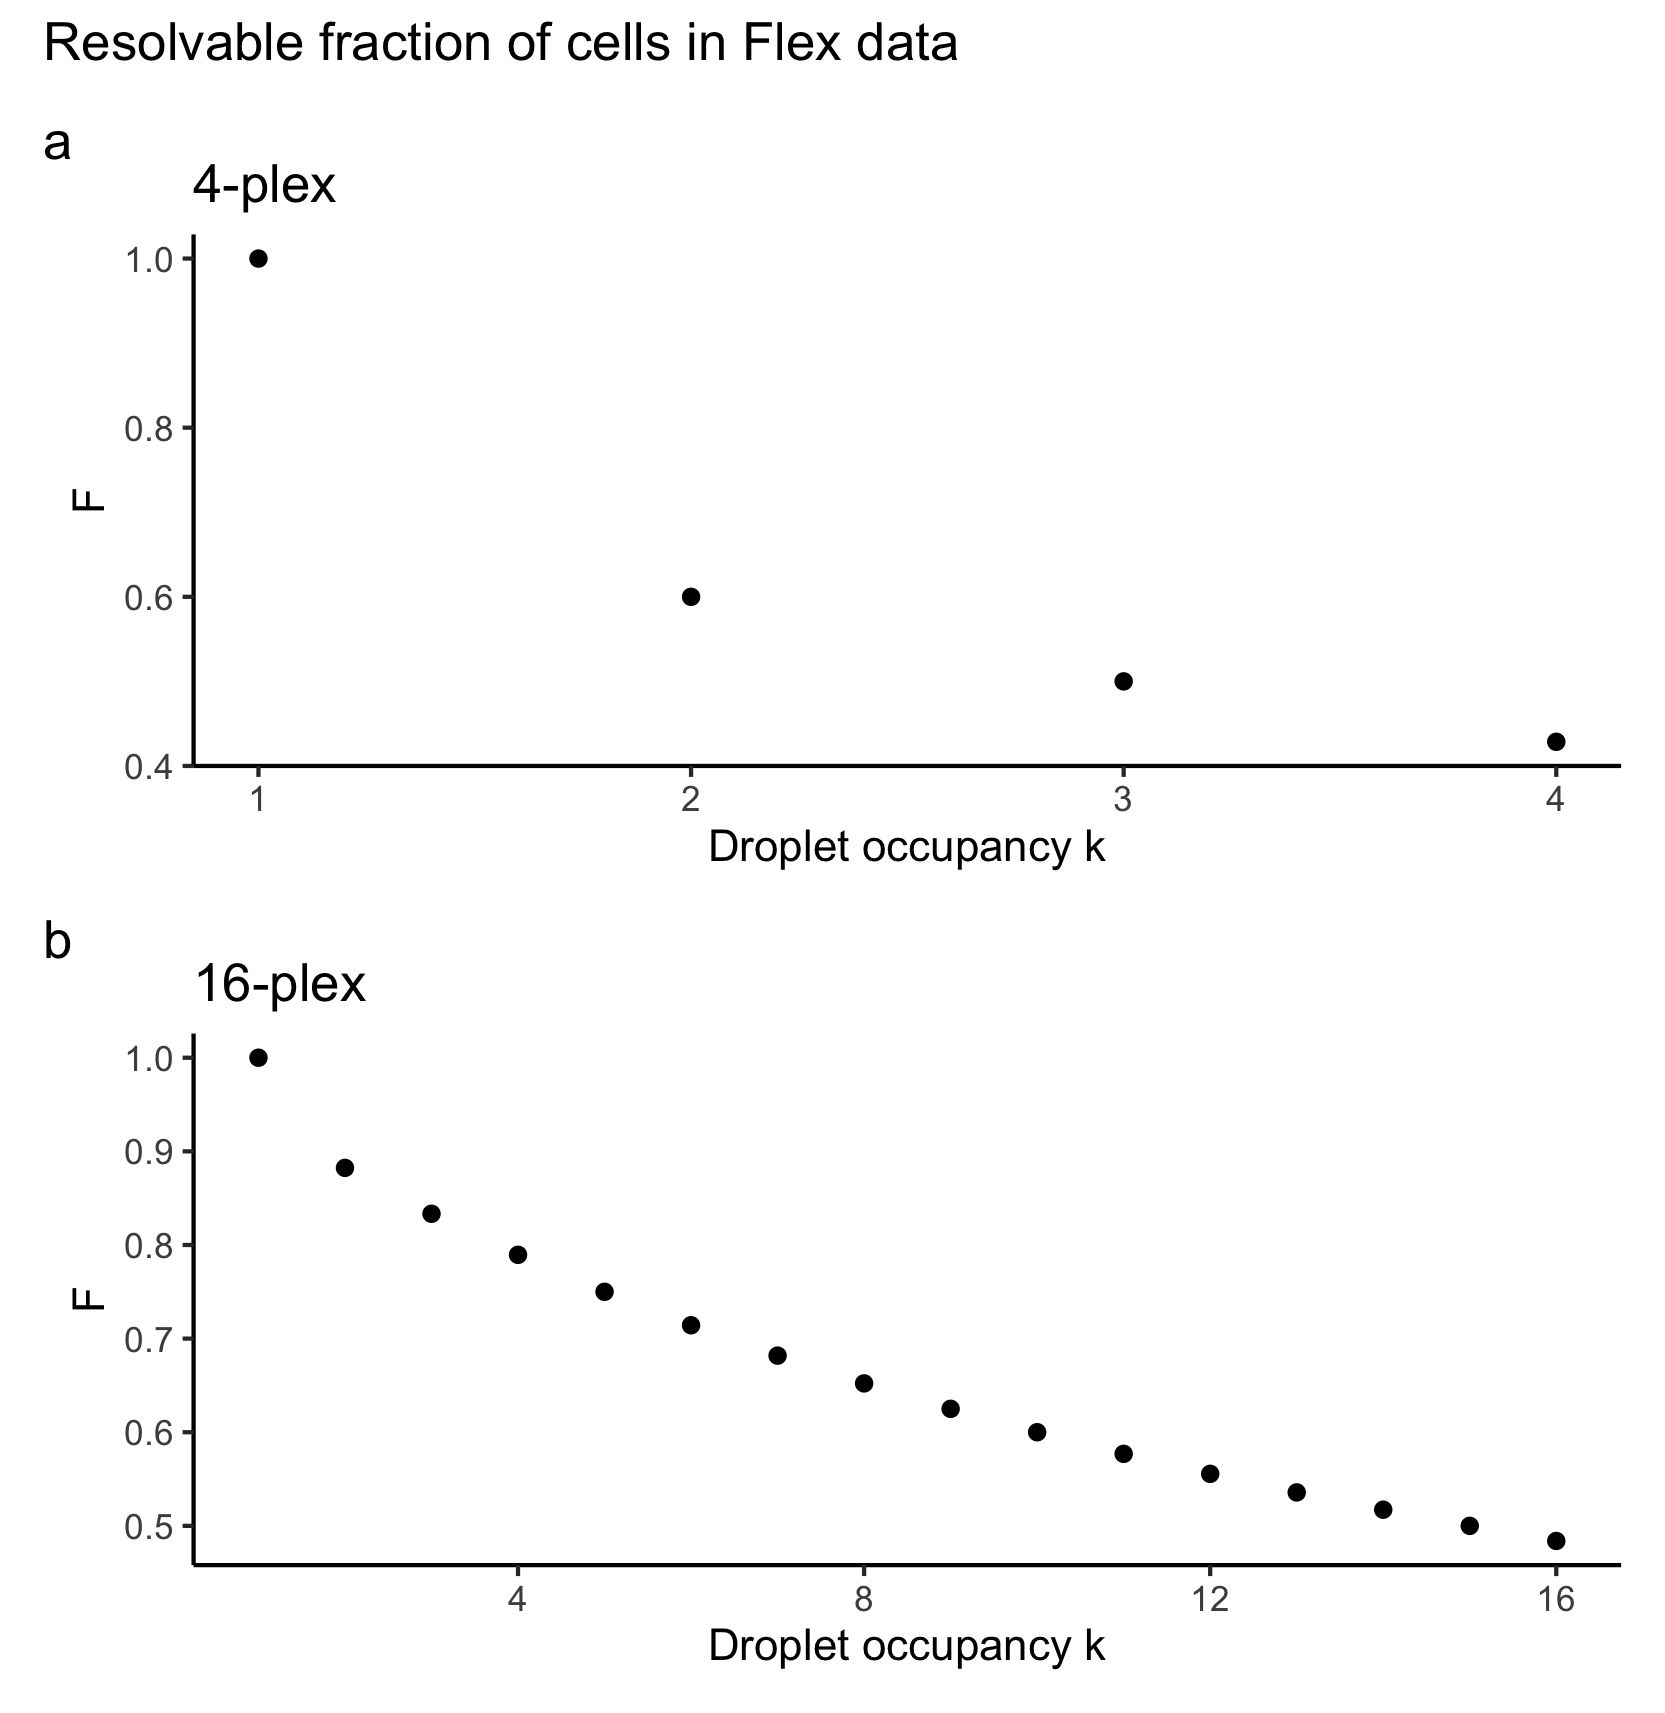
\includegraphics[scale=0.1]{figures/observable_fraction_GEM_occupancy.png}
			\caption{Fraction of resolvable cells $F(n, k)$ vs occupancy $k$ for (a) $n = 4$ and (n) $n = 16$.
			}		
			\label{fig:resolvable_fraction}
		\end{center}
	\end{figure}
	%
	Figure \ref{fig:resolvable_fraction} shows that $F$ decreases steeply with $k$, with $F(n = 4) < 0.5$,  for $k > 2$ and $F(n = 16) < 0.75$ for $k > 5$.
	
	To determine the size of the effect in real data, we need to combine equation \eqref{eq:resolvable fraction} with the distribution of droplet occupancy $k$. 
	A good model for the distribution of observed occupancy $l$ in Flex data is the zero-truncated Poisson distribution, as zeros, or empty droplets, are not included in the CellRanger output (Supplementary Figure 1)
	%
	\begin{equation}
		p(l) = \frac{\lambda^l}{l! (e^{\lambda} - 1)}  ,
		\label{eq: poisson_distribution} 
	\end{equation}
	%
	where $\lambda$ is a shape parameter related to the mean droplet occupancy $\langle l \rangle$ through
	%
	\begin{equation}
		\langle l \rangle = \frac{\lambda}{1 - e^{- \lambda}}  .
		\label{eq: poisson expectation value}
	\end{equation}
	% 
	We now make a simplifying assumption that the distribution of the true occupancy $k$ can be approximated by the distribution of the observed occupancy $l$, i.e.
	%
	\begin{equation}
		p(k) \approxeq p(l)  .
		\label{eq:pdf approximation}
	\end{equation}
	%
	We make this assumption in order to simplify what follows, and because determination of a relationship between $k$ and $l$ is a non-trivial task requiring a more robust ground-truth data set for known doublets in Flex data than is currently available. 
	The number of cells in droplets with observed occupancy $k$ is then 
	%
	\begin{equation}
		N_{\rm cells}(k) = N_{\rm droplets} k p(k).
		\label{eq:cells_at_occupancy}
	\end{equation}
	%
	Combining  equations \eqref{eq:resolvable fraction} -- \eqref{eq:cells_at_occupancy}, we get the fraction of multiplets in an experiment 
	%
	\begin{equation}
		M_f(n) = 1 - \sum_k \frac{k p(k) F_{\rm r}(n, k)}{\langle l \rangle} \quad .
		\label{eq:dataset resolvable fraction}
	\end{equation}
	%
	We show the expected doublet fraction in data sets for $n = 4$ and $n = 16$ as a function of mean observed droplet occupancy $\langle l \rangle$ in Figure \ref{fig: resolvable fraction observed}.
	Figure \ref{fig: resolvable fraction observed} also includes the doublet fraction from scDblFinder for the earlyAIR and PBMC data sets in the 16-plex case 
	\citep{Germain2021}.
	%
	\begin{figure}
		\begin{center}
			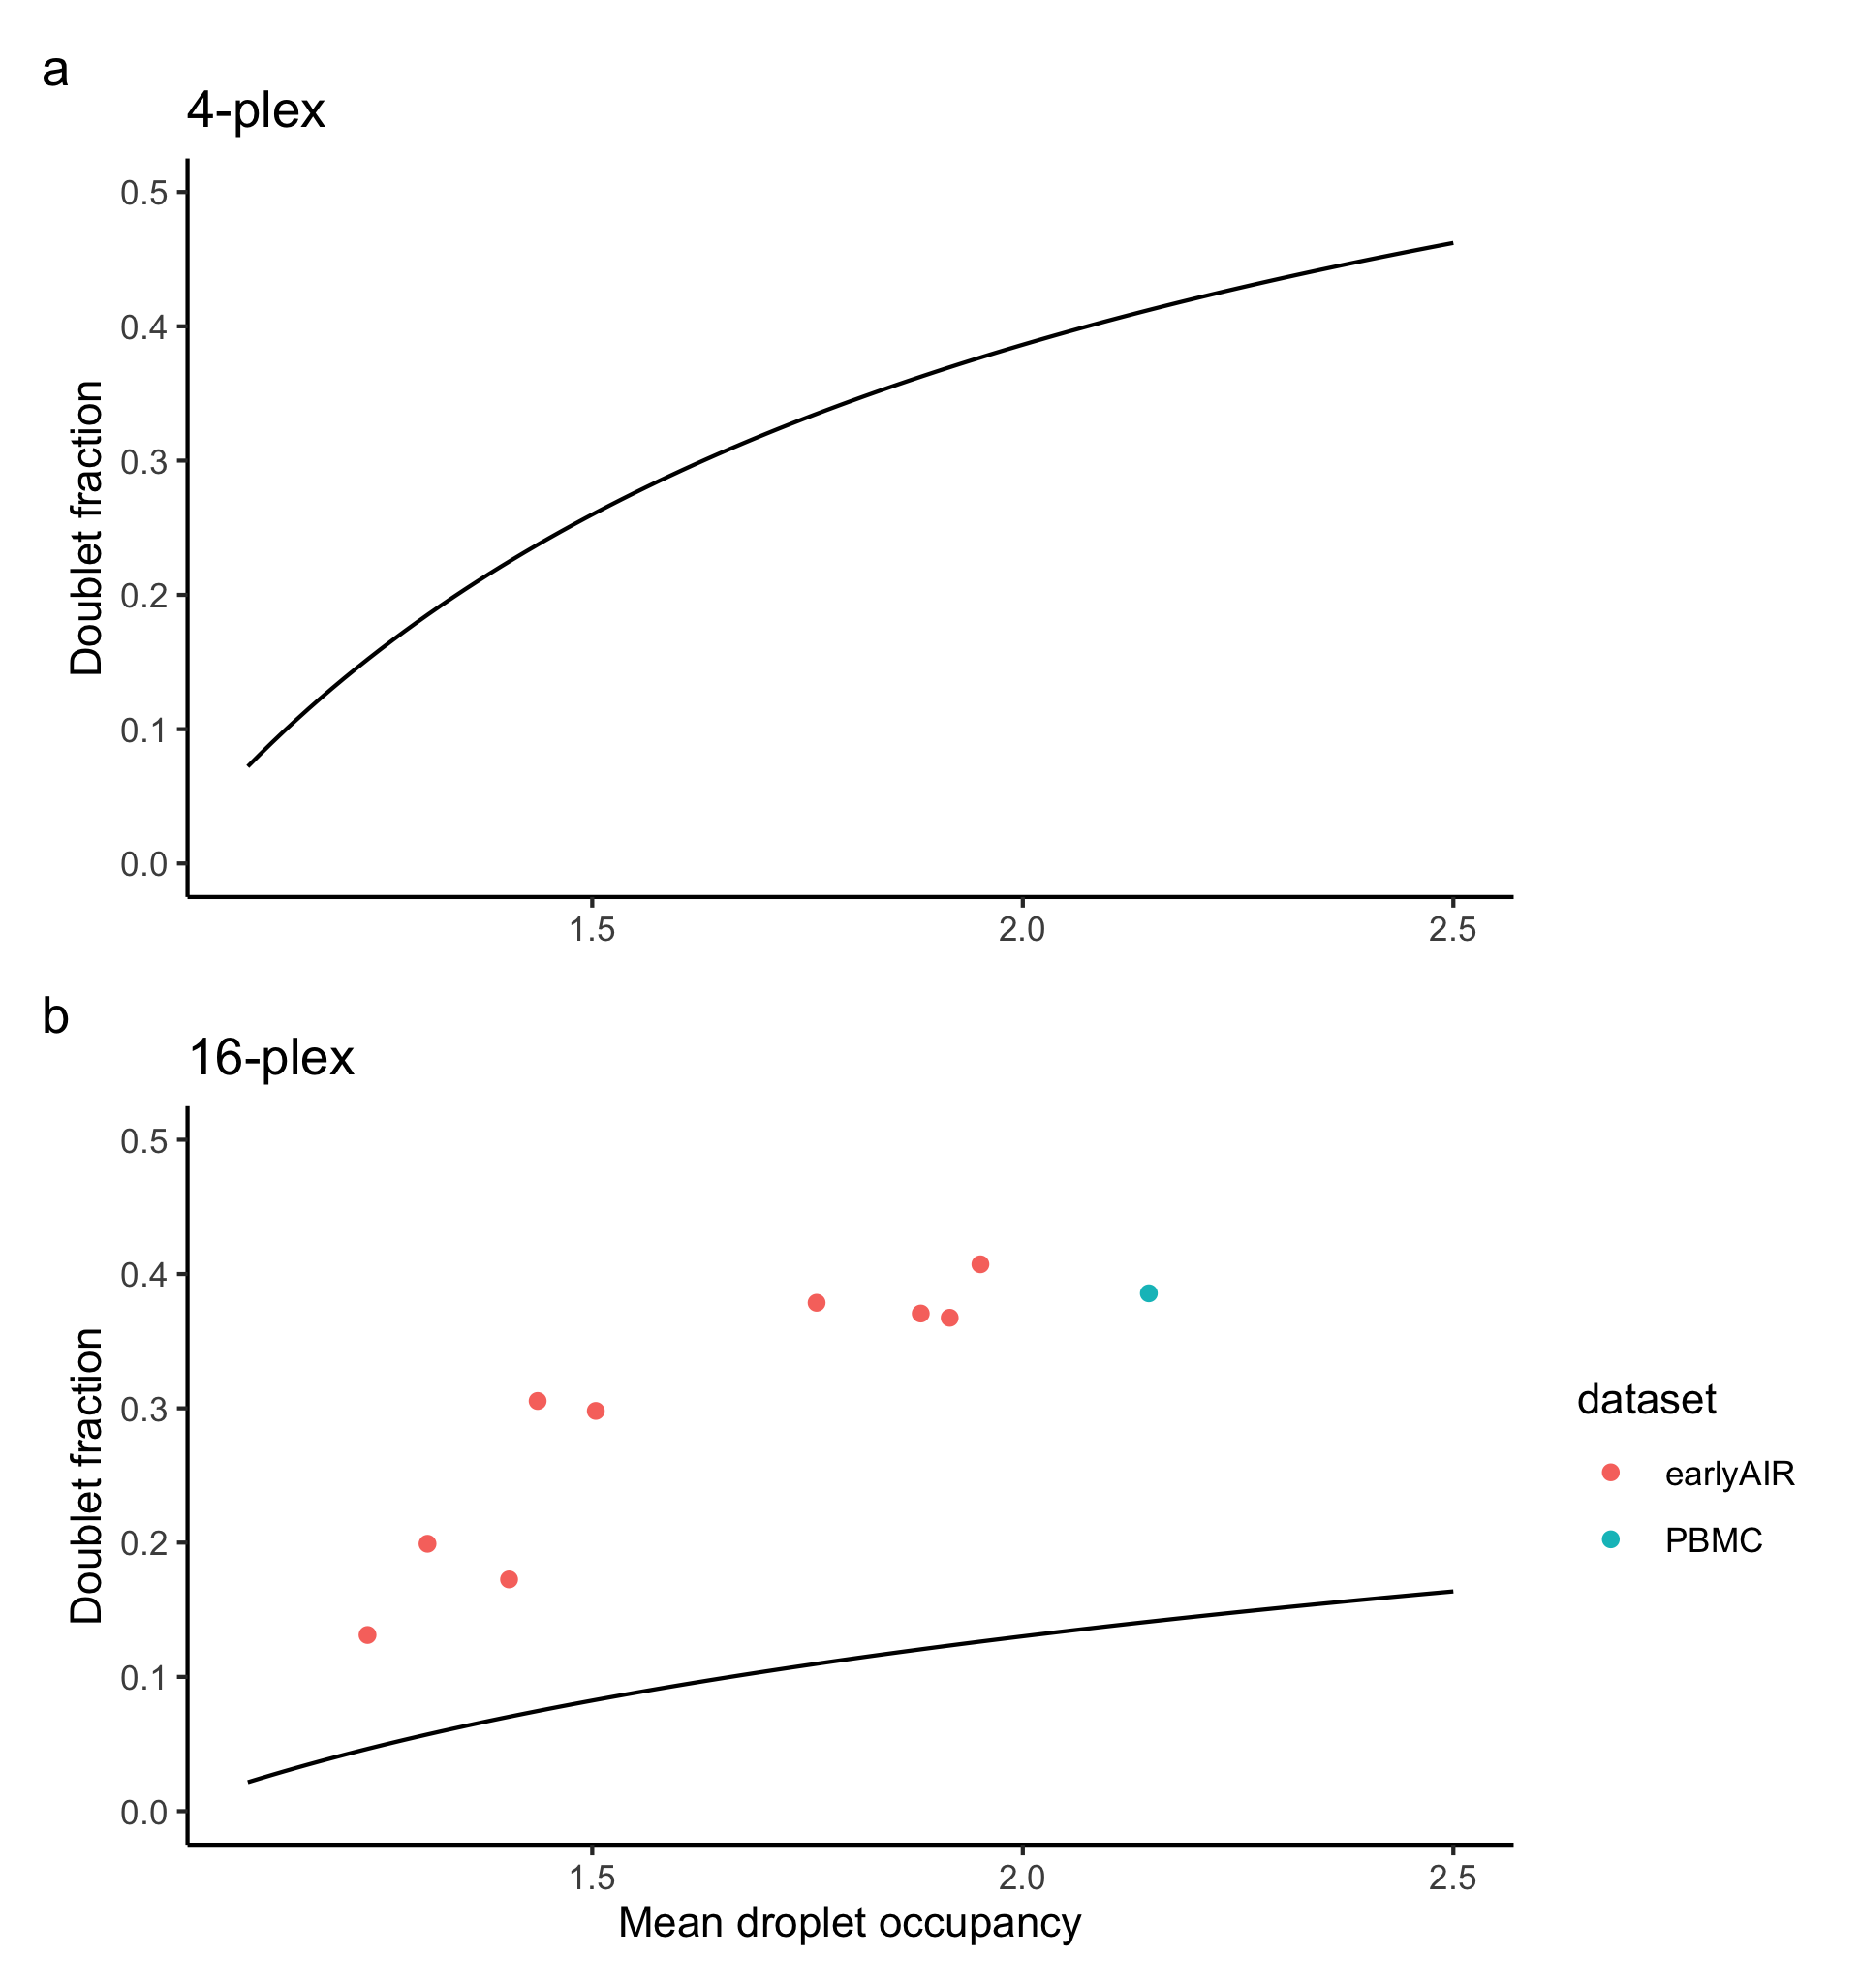
\includegraphics[scale=0.1]{figures/observable_fraction.png}	
			\caption{Calculated fraction of multiplets in Flex data vs mean droplet occupancy given the number of multiplexed samples a) $n = 4$ and b) $n = 16$.
			Coloured points indicate doublet fraction determined from scDblFinder and observed mean droplet occupancy from earlyAIR and PBMC data sets.
			}		
			\label{fig: resolvable fraction observed}
		\end{center}
	\end{figure}
	%		
	Figure \ref{fig: resolvable fraction observed} shows that the predicted multiplet fraction from equation \eqref{eq:dataset resolvable fraction} still underestimates the doublet fraction we observe in real-world data, though by significantly less than the prediction from the Flex User Guide 
	\citep{10X_flex_protocol}. 
	We propose two potential reasons for this discrepancy. 
	The first is the assumption that the true occupancy distribution is the same as the observed distribution, equation \ref{eq:pdf approximation}.
	The presence of unresolvable cells implies that the true occupancy is always greater than that observed, see Supplementary Figure 3.
	%
%	\begin{figure}
%		\begin{center}
%			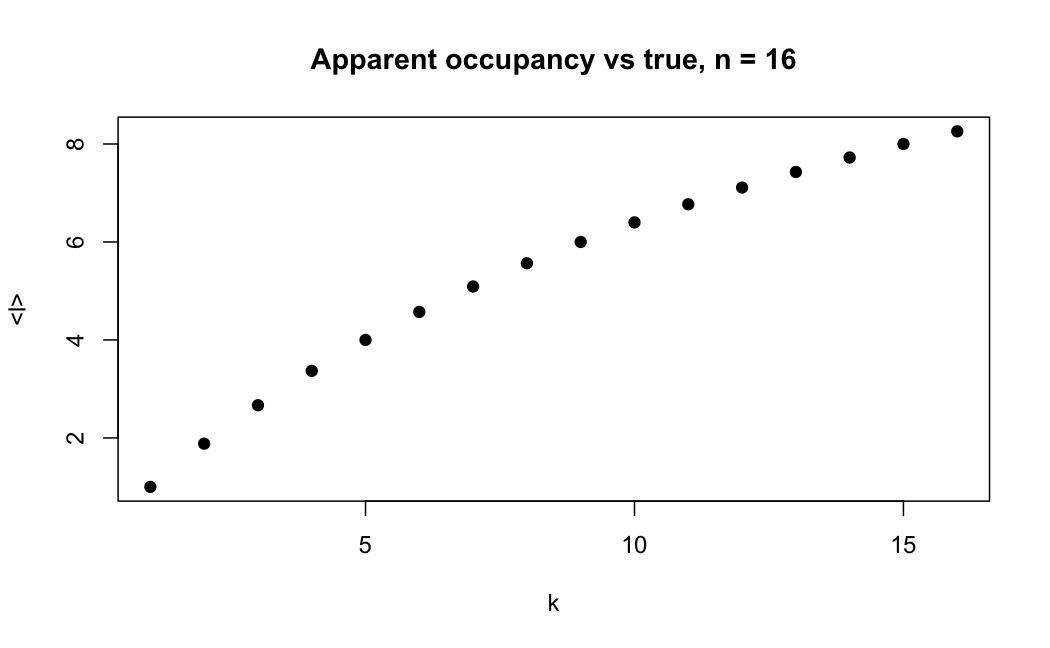
\includegraphics[scale=0.2]{figures/mean_l_vs_k.png}
%			\caption{Probability of observed occupancy $l$ given true occupancy $k$.
%			}		
%			\label{fig:mean l vs k}
%		\end{center}
%	\end{figure}
	%
	 Properly accounting for this effect would shift the data points in Figure \ref{fig: resolvable fraction observed} to the right, bringing them closer to the predicted curve. 	
	Another reason is the assumption that all samples have equal numbers of cells. 
	In any experiment, some samples contain more cells than others. We expect that this increases the likelihood of same-sample multiplets, though exactly how is beyond the scope of this work. 
	
	Even with the limiting assumptions of our model, however, the fraction of unresolved multiplets in an experiment with a mean droplet occupancy of 2.5 (a typical value for an experiment with the maximum recommended loading of 128,000 cells) is 0.17, almost 3 times greater than the value of 0.064 estimated by 10X. These results demonstrate the necessity of removing doublets from Flex data. 
		
	Finally, in Figure \ref{fig:doublet_finder_comparison}b we observe that scDblFinder calls 2060 of the droplets in the PBMC data set identified as singlets by CellRanger as doublets. 
	We can estimate the number of observed singlets that are actually doublets using equation \eqref{eq:resolvable fraction} and the observed distribution of droplet occupancies. 
	From this, we estimate that $\sim$ 2700 droplets with occupancy $k > 1$ will appear as singlets in this data set. 
	Most of these will have $k=2$ (2 cells, 2400 droplets), but some droplets can contain more cells from the same sample (Supplementary Figure 2). 
	The number predicted by the model is similar to the value of 2,060 from scDblFinder, with the discrepancy likely due to the difficulty of scDblFinder in identifying homotypic doublets, shown in Figures \ref{fig:doublet_finder_comparison}b) and e).
	
	\subsection{Doublet-finding identifies spurious clusters}
	
	In order to demonstrate the effect of doublets on downstream analysis, we perform unsupervised clustering on the PBMC data set at a range of resolutions from 0.1 to 1.0 using the \texttt{FindMarkers} function with the SLM algorithm in Seurat.
	We use two versions of the data: (1) all cells that pass our initial QC filtering, and (2) after removing all of the doublets identified by scDblFinder. 
	At every resolution, removing the doublets reduces the number of clusters (Figure \ref{fig:doublet_clusters}a), indicating that doublets introduce structure in the data. 
	% 
	\begin{figure*}
		\begin{center}
			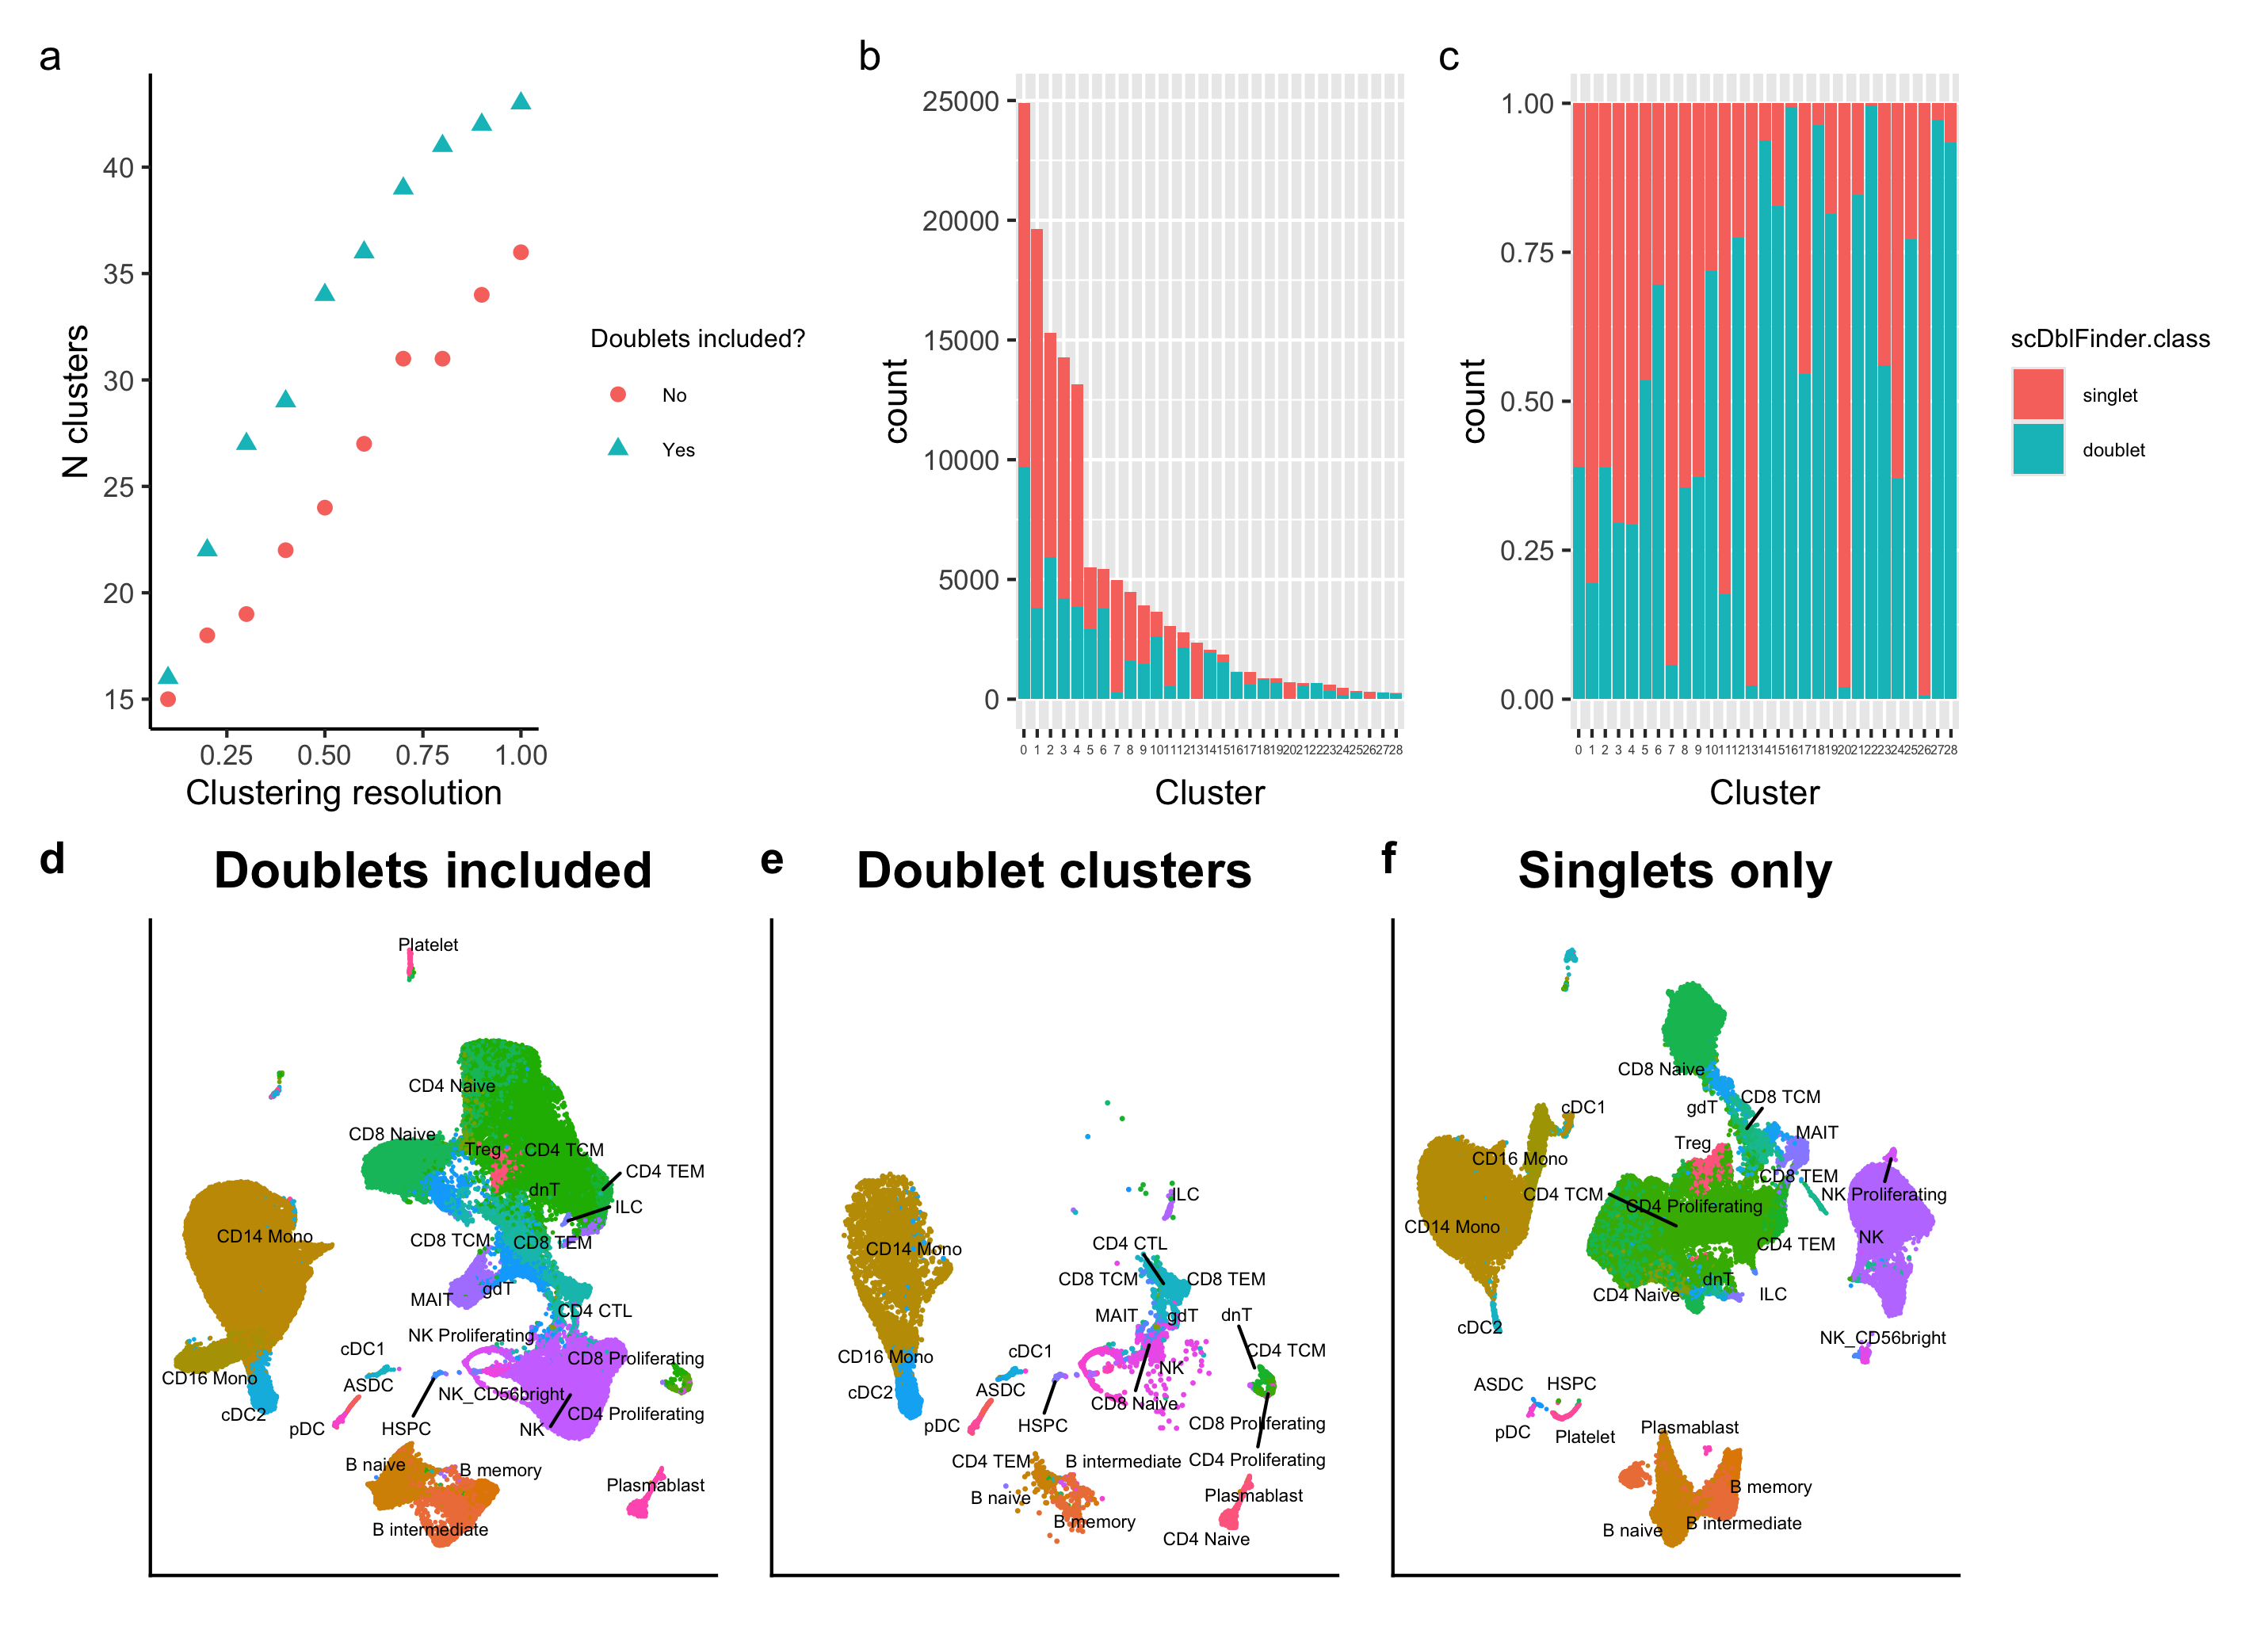
\includegraphics[scale=0.15]{figures/doublet_QC.png} 
			\caption{ 
				a) Number of clusters as a function of cluster resolution for PBMC data set before (blue triangles) and after (red circles) removal of doublets identified by scDblFinder. 
				b) Number of cells in each cluster in the PBMC data set at resolution 0.4, coloured by fraction of doublets. 
				c) same as b) but with proportions instead of total counts. 
				d) UMAP showing cells in the PBMC data set with labels from Azimuth. 
				e) Same as d) but showing only cells from clusters with $\geq 75\%$ doublets. 
				f) UMAP with Azimuth labels computed after removing doublets.
				}
			\label{fig:doublet_clusters}
		\end{center}	
	\end{figure*} 
		
	We next look at the doublet composition of the identified cluster at resolution 0.4, (Figures \ref{fig:doublet_clusters}b and c). 
	We identify 11 clusters that contain more than twice the average doublet fraction of the entire data set. 
	 We show the position of all cells in the data set prior to doublet removal, las annotated by Azimuth, on a Uniform Manifold Approximation and Projection (UMAP) plot in Figure \ref{fig:doublet_clusters}d. 
	 Figure \ref{fig:doublet_clusters}e shows only the cells in the 11 clusters identified as being composed of mostly doublets.
	 Figures \ref{fig:doublet_clusters}d and e show that these doublet-dominated clusters appear in the regions of the UMAP that bridge multiple cell types, such as CD14 and CD16 monocytes, or T cells and NK cells, lending further evidence for their identity as doublets. 
	 Version (1) of the PBMC data  contains 52,336 more cells than version (2), which may be responsible for the greater number of clusters. 
	 To check this, we randomly remove an equivalent number of cells as the number of doublets from version (1) , so that the resulting data set has the same number of cells as (2) with the same singlet/doublet ratio as (1). 
	 After repeating this process 10 times we find that in general, the downsampled data sets contain fewer clusters than (1) but more than (2), and that a significant proportion of clusters are dominated by doublets (see Supplementary Figure 3).	 
	 
	 Lastly, Figure  \ref{fig:doublet_clusters}f shows the UMAP with Azimuth labels after removing the doublets. 
	 In Figure  \ref{fig:doublet_clusters}f, certain cell populations, such as T and NK cells, CD4 T cells and CD8 T cells, and CD14 and CD16 Monocytes, are better separated in more distinct clusters than in Figure  \ref{fig:doublet_clusters}d.
	
	\section{Discussion}
	\label{sec:discussion}
	
	Sample barcoding, as implemented in the 10X Flex protocol, offers a solution to two significant issues in droplet-based scRNA-seq experiments: robust identification of sample-of-origin in multiplexed cell pools, and deconvolution of multiple cells from different samples in the same droplet. 
	However, herein we demonstrate that unresolvable doublets, consisting of multiple cells from the same sample, remain a significant issue in Flex data sets, with scDblFinder classifying several times more cells as doublets than predicted by the manufacturer. 
	
	Despite the greater-than-expected number of doublets in Flex data, we find that in general the Flex protocol provides similar data quality to previous 3’ scRNA-seq protocols, and existing tools and workflows, such as ambient RNA removal and cell annotation, work without issue. 
	This includes doublet finders previously developed for 3' data sets.
		
	We verify that the predictions of scDblFinder are accurate by aggregating the droplet counts across the sample barcodes, a novel approach that will prove useful in future benchmarking studies of doublet-finding algorithms. 
	We then propose a mathematical model for predicting the number of same-sample doublets in any droplet-based single-cell protocol with sample barcodes, and find that the predictions of our model are much closer to the observed doublet rates in Flex experiments than the estimates from the user documentation. 
	Importantly, we demonstrate that doublet removal improves downstream analysis by eliminating spurious cell clusters consisting primarily of doublets.
	
	
	\section{Methods}
	\label{sec:methods}
	
	\subsection{Single-cell data generation}
	\label{subsec:data_generation}
	
	For the earlyAIR data set, samples were processed to single-cell suspensions, fixed within 1 hour of collection according to 10x Genomics Flex Protocol recommendations 
	\citep{10X_flex_protocol}
	and stored at -80C until enough samples for one batch of 16 had been collected. 
	Samples were thawed, barcoded, pooled (16 samples per pool), and processed according to 10x Genomics recommendations without modifications. Fo
	r each capture, 128,000 cells were targeted, libraries were prepared using standard protocols, and sequencing was performed to achieve 10,000 reads/cell.	
	
	\subsection{Single-cell data pre-processing strategy}
	\label{subsec:preprocessing}
	
	The starting point for all data sets discussed in this paper is a counts matrix consisting of cells called by CellRanger. This data is pre-processed in the following order prior to running doublet-finding tools. 
	%
	\begin{itemize}
		\item Removal of unexpressed genes.
		\item Removal of ambient background contamination using decontX 
		\citep{Yang2020}.
		\item Removal of cells with fewer than 250 reads.
		\item Removal of cells with high mitochondrial read percentages, using the \texttt{isOutlier} function in the \texttt{DropletUtils} package
		\citep{Griffiths2018, Lun2019}.		
		\item Doublet calling with scDblFinder
		\citep{Germain2021}
	\end{itemize} 
	%
	
	\subsection{Overview of doublet-finding tools}
	
	We test two doublet-finding tools on the droplet-level counts for the PBMC data set, scds and scDblFinder. 
	scds 
	\citep{Bais2020}
	has two methods for doublet detection, the coexpression method and the binary classification. 
	The co-expression method assigns a score to every pair of genes based on how often they are expressed in the same droplets. 
	This score is aggregated across all pairs for each droplet to create a doublet score, which is higher for droplets that co-express gene pairs with a low co-expression score. The binary classification method generates artificial doublets by adding random pairs of columns in the counts matrix and creating an augmented data set consisting of the input data and the artificial doublets. 
	A classifier for distinguishing the input data from the artificial doublets is trained on the combined data set using boosted decision trees, and then run on the input data alone to compute a doublet score for each droplet. scds can also compute a hybrid score which is the average of the scores from the co-expression and binary classification methods, and droplets are called either singlets or doublets based on a threshold determined from the expected number of doublets in the data set.
	
	scDblFinder 
	\citep{Germain2021}works similarly to the binary classification method in scds but rather than using the counts matrix directly, artificial doublets are generated in a lower dimensional representation of the expression space and creating a k-nearest neighbours graph.
	scDblFinder runs for several iterations, removing the input droplets with the highest doublet scores and regenerating the artificial doublets at each iteration. 		
	
	
	%%%%%%%%%%%%%%
	
	\section{Data availability}
	\label{sec:data availability}
	
	
	
	\section{Acknowledgments}
	\label{acknowledgements}
	
	Data generation for the earlyAIR data set was performed by WEHI’s Cellular Genomics Projects Team, with sequencing performed by Stephen Wilcox and Sarah MacRaild and additional data generation by Casey J. A. Anttila and Ruvimbo Mishi.
	We thank Professor Andrew Melatos for suggesting using partitions as a way to describe the distribution of cells within droplets. 
	
	This project is supported by CZI Pediatric Networks for the Human Cell Atlas 2021-237883.
	AO is supported by NHMRC Investigator grant (GNT1196256). 
	JM is supported by NHMRC Investigator grant (GNT1187748). CZI funding 
	
	
	\bibliographystyle{plain}
	\bibliography{flex_multiplets} 
	
	
	%USE THE BELOW OPTIONS IN CASE YOU NEED AUTHOR YEAR FORMAT.
	%\bibliographystyle{abbrvnat}
	
	
	
\end{document}
